% !TeX root = proyecto.tex
%=========================================================
\chapter{Modelo de la interacción}	
\label{cap:modInteraccion}

\cdtInstrucciones{Introduzca el capítulo indicando su contenido y organización.}	

\cdtInstrucciones{Utilice este capítulo para describir todos los detalles de la interacción con el usuario, describiendo elementos d eusabilidad, ergonomía, psicología,  arqjuitectura de información y repreentación.}

Este capítulo describe ...

\section{Modelo de navegación}

\cdtInstrucciones{Describa de acuerdo al tipo de aplicación como es la interacción con el usuario, destacando los elementos de ubicación dentro de la aplicación. Si las interfaces tiene elementos comunes más allá de los que son comunes a todas las aplicaciones describalos ampliamente así como los encabezados, pies de página, menús y otros elementos que aparecen repetitivamente entre las pantallas.}

	La navegación entre pantallas se muestra en la figura~\ref{fig:mapa}. en el se explica ...\\

\begin{figure}[htbp]
	\begin{center}
		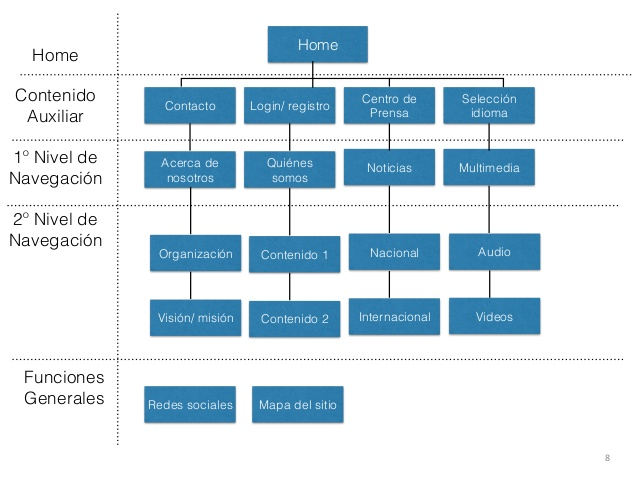
\includegraphics[width=.7\textwidth]{images/mapa}
		\caption{mapa}
		\label{fig:mapa}
	\end{center}
\end{figure}


\cdtInstrucciones{A continuación describa cada una de las pantallas.}
% !TeX root = ../proyecto.tex
%--------------------------------------
\section{IUX Interfaz (nombre de la interfaz)}

\subsection{Objetivo}
	\cdtInstrucciones{Describa el objetivo, propósito o función de la pantalla.}

\subsection{Diseño}
	\cdtInstrucciones{Describa brevemente los elementos de la pantalla y como de be usarse a manera de manual de usuario.} Esta pantalla \IUref{IU23}{Pantalla de Control de Acceso} aparece al iniciar el sistema, para ingresar ... 

\IUfig[.7]{Login}{IU23}{Pantalla de Control de Acceso.}

%\IUfig[ancho de la figura: valor entre 1 y .1]{Nombre corto de la pantalla sin espacions ni acentos}{IUXX}{Nombre largo de la pantalla.}

\subsection{Salidas}

	\cdtInstrucciones{Liste las salidas de la interfaz. Si coinciden con las del caso de uso solo indiquelo. Esta ,ista debe incluir los mensajes}

	\begin{itemize}
		\item Descripción de salida.
	\end{itemize}
	
\subsection{Entradas}

	\cdtInstrucciones{Liste las entradas de la interfaz. Si coinciden con las del caso de uso solo indiquelo.}
	\begin{itemize}
		\item Descripción de salida.
	\end{itemize}

\subsection{Comandos}
	\cdtInstrucciones{Describa cada control (botónes, areas de drag and drop, componentes interactivos, animaciones, etc.) que se puede utilizar dentro de la pantalla indicando o que hacen y si cambia de pantalla.}

\begin{itemize}
	\item \IUbutton{Entrar}: Verifica que el Estudiante se encuentre registrado y la contraseña sea la correcta. Si la verificación es correcta, se muestra la \IUref{UI32}{Pantalla de Selección de Seminario}.
	\item \IUbutton{Ayuda}: Muestra la ayuda de esta pantalla \IUref{IU50}{Pantalla de Ayuda}.
\end{itemize}



%!TEX root = ejemplo.tex
%=========================================================
\section{Catálogo de mensajes}	
\label{sec:mensajes}

	En esta sección se describen todos los mensajes que aparecen en el sistema. Para cada mensaje se especifica:
	 
	\begin{description}\itemsep0em
		\item[Id:] Identificador del mensaje de la forma ``MSG XX'' y descripción corta del mismo.
		\item[Tipo:] Tipo del mensaje el cual puede ser: 
		\begin{description}
			\item[Normal:] Mensaje que informa al usuario una instrucción o el estado interno que guarda el sistema, suele tener un color {\color{msgNormalColor}Azul}.
			\item[Éxito:] Mensaje que informa al usuario sobre una acción realizada, sirve para confirmar el correcto funcionamiento del sistema. Se presentan con un color {\color{msgInfoColor}Verde}.
			\item[Atención:] Mensaje que tiene como finalidad llamar la atención del usuario a una situación que requiere su intervención, por ejemplo cuando una actividad ha generado un efecto colateral o se realizará una acción destructiva y no reversible. Se presentan con un color {\color{msgWarningColor}Naranja}.
			\item[Error:] Mensaje que informa al usuario un fallo en en una operación o un impedimento para realizarla, por ejemplo: cuando no se puede efectuar la acción solicitada, cuando un dato falta o tiene un formato no aceptado por el sistema. Se presentan con un color {\color{msgErrorColor}Rojo}.
		\end{description}
		\item[Propósito:] Explicación del propósito del mensaje.
		\item[Redacción:] Redacción del mensaje.
		\item[Parámetros:] En caso de que el mensaje pueda variar se especifican los casos y la forma en que debe adaptarse la redacción
		\item[Ejemplos:] Ejemplos de como debe renderizarse el mensaje.
	\end{description}


\subsection{Lista de mensajes}

%msgNormalColor
%msgInfoColor
%msgWarningColor
%msgErrorColor
\begin{cdtMessage}[msgInfoColor]{MSG-001}{Bienvenida al usuario}
	\item[Propósito:] Indicar al usuario que ha ingresado satisfactoriamente al sistema.
	\item[Redacción:] Bienvenido $<$nombre$>$.
	\item[Parámetros:] \hspace{1cm}
	\begin{itemize}
		\item $<$nombre$>$ \hyperlink{Usuario.nombre}{Nombre completo} del Usuario.
	\end{itemize}
	\item[Ejemplos:] Bienvenido Juan Pérez.
\end{cdtMessage}

%msgNormalColor
%msgInfoColor
%msgWarninigColor
%msgErrorColor
\begin{cdtMessage}{MSG-002}{Usuario no registrado} 
	\item[Propósito:] Indica que el usuario ingresado no existe en el sistema.
	\item[Redacción:] El usuario $<$login$>$ no se encuentra registrado.
	\item[Parámetros:] \hspace{1cm}
	\begin{itemize}
		\item $<$login$>$ \hyperlink{Usuario.login}{Login} del Usuario.
	\end{itemize}
	\item[Ejemplos:] El usuario juanP no se encuentra registrado.
\end{cdtMessage}

%msgNormalColor
%msgInfoColor
%msgWarninigColor
%msgErrorColor
\begin{cdtMessage}[msgErrorColor]{MSG-003}{Cuenta inactiva} 
	\item[Propósito:] Indicar al usuario que la cuenta especificada se encuentra inactiva.
	\item[Redacción:] La cuenta especificada $<$login$>$ se encuentra inactiva, favor de contactar al Secretario Escolar para mas información.
	\item[Parámetros:] \hspace{1cm}
	\begin{itemize}
		\item $<$login$>$ \hyperlink{Usuario.login}{Login} del Usuario.
	\end{itemize}
	\item[Ejemplos:] La cuenta especificada juanP se encuentra inactiva, favor de contactar al Secretario Escolar para mas información.
\end{cdtMessage}

%msgNormalColor
%msgInfoColor
%msgWarninigColor
%msgErrorColor
\begin{cdtMessage}[msgErrorColor]{MSG-004}{Error de inicio de sesión}
	\item[Propósito:] Indica al usuario que la contraseña introducida es incorrecta.
	\item[Redacción:] La contraseña ingresada es incorrecta.
	\item[Parámetros:] No aplica.
	\item[Ejemplos:] La contraseña ingresada es incorrecta.
\end{cdtMessage}

%msgNormalColor
%msgInfoColor
%msgWarninigColor
%msgErrorColor
\begin{cdtMessage}{MSG-008}{Tiempo restante para terminar un proceso} 
	\item[Propósito:] Indicar al usuario el tiempo restante para terminar una operación limitada en el tiempo como la reinscripción.
	\item[Redacción:] Quedan $<$tiempo$>$ para terminar la $<$operación$>$.
	\item[Parámetros:] \hspace{1cm}
	\begin{itemize}
		\item $<$tiempo$>$ Tiempo faltante para la operació especificando días, horas minutos y segundos.
		\item 
	\end{itemize}
	\item[Ejemplos:] \hspace{1cm}
	\begin{itemize}
		\item Quedan 45 días, 2 horas 12 minutos y 45 segundos para iniciar tu reinscripción.
		\item Quedan 2 minutos y 32 segundos para terminar tu reinscripción
	\end{itemize}
\end{cdtMessage}

\begin{cdtMessage}[msgInfoColor]{MSG-009}{Operación exitosa}
	\item[Propósito:] Informar al usuario que la operación solicitada ha sido ejecutada con éxito.
	\item[Redacción:] $<$Artículo$>$ $<$Operación$>$ del $<$Entidad$>$ $<$Identificador$>$ se realizó con éxito.
	\item[Parámetros:]\hspace{1pt}
	\begin{itemize}
		\item $<$Artículo$>$ $<$Operación$>$ se refiere a la operación realizada.
		\item $<$Entidad$>$ $<$Identificador$>$ se refiere al elemento del negocio donde recayó la operación, indicando el tipo del objeto y un dato que el usuario pueda usar para identificarlo.
	\end{itemize}
	\item[Ejemplo:] Algunos ejemplos son
	\begin{itemize}
		\item El registro del Alumno 342343 se realizó con éxito.
		\item La eliminación de la Tarea ``documentar el proceso'' se ha realizado con éxito.
	\end{itemize}
\end{cdtMessage}
